\documentclass[]{article}

% Imported Packages
%------------------------------------------------------------------------------
\usepackage{amssymb}
\usepackage{amstext}
\usepackage{amsthm}
\usepackage{amsmath}
\usepackage{enumerate}
\usepackage{fancyhdr}
\usepackage[margin=1in]{geometry}
\usepackage{graphicx}
%\usepackage{extarrows}
%\usepackage{setspace}
\graphicspath{ {../images/} }
%------------------------------------------------------------------------------

% Header and Footer
%------------------------------------------------------------------------------
\pagestyle{plain}  
\renewcommand\headrulewidth{0.4pt}                                      
\renewcommand\footrulewidth{0.4pt}                                    
%------------------------------------------------------------------------------

% Title Details
%------------------------------------------------------------------------------
\title{Deliverable \#2 Template}
\author{SE 3A04: Software Design II -- Large System Design}
\date{}                               
%------------------------------------------------------------------------------

% Document
%------------------------------------------------------------------------------
\begin{document}

\maketitle
\noindent{\bf Tutorial Number:} T03\\
{\bf Group Number:} G06 \\
{\bf Group Members:}
\begin{itemize}
	\item Virochaan Ravichandran Gowri
	\item Alex Yoon
	\item Noah Goldschmied
	\item Krish Dogra
	\item Leo Vugert
\end{itemize}

\section*{IMPORTANT NOTES}
\begin{itemize}
	%	\item You do \underline{NOT} need to provide a text explanation of each diagram; the diagram should speak for itself
	\item Please document any non-standard notations that you may have used
	      \begin{itemize}
		      \item \emph{Rule of Thumb}: if you feel there is any doubt surrounding the meaning of your notations, document them
	      \end{itemize}
	\item Some diagrams may be difficult to fit into one page
	      \begin{itemize}
		      \item Ensure that the text is readable when printed, or when viewed at 100\% on a regular laptop-sized screen.
		      \item If you need to break a diagram onto multiple pages, please adopt a system of doing so and thoroughly explain how it can be reconnected from one page to the next; if you are unsure about this, please ask about it
	      \end{itemize}
	\item Please submit the latest version of Deliverable 1 with Deliverable 2
	      \begin{itemize}
		      \item Indicate any changes you made.
	      \end{itemize}
	\item If you do \underline{NOT} have a Division of Labour sheet, your deliverable will \underline{NOT} be marked
\end{itemize}

\newpage
\section{Introduction}
\label{sec:introduction}
% Begin Section

This section should provide an brief overview of the entire document.

\subsection{Purpose}
\label{sub:purpose}
% Begin SubSection
State the purpose and intended audience for the document.
% End SubSection

\subsection{System Description}
\label{sub:system_description}
% Begin SubSection
Give a brief description of the system. This could be a paragraph or two to give some context to this document.

% End SubSection

\subsection{Overview}
\label{sub:overview}
% Begin SubSection
Describe what the rest of the document contains and explain how the document is organised (e.g. "In Section 2 we discuss...in Section 3...").

% End SubSection

% End Section

\section{Analysis Class Diagram}
\label{sec:analysis_class_diagram}
% Begin Section
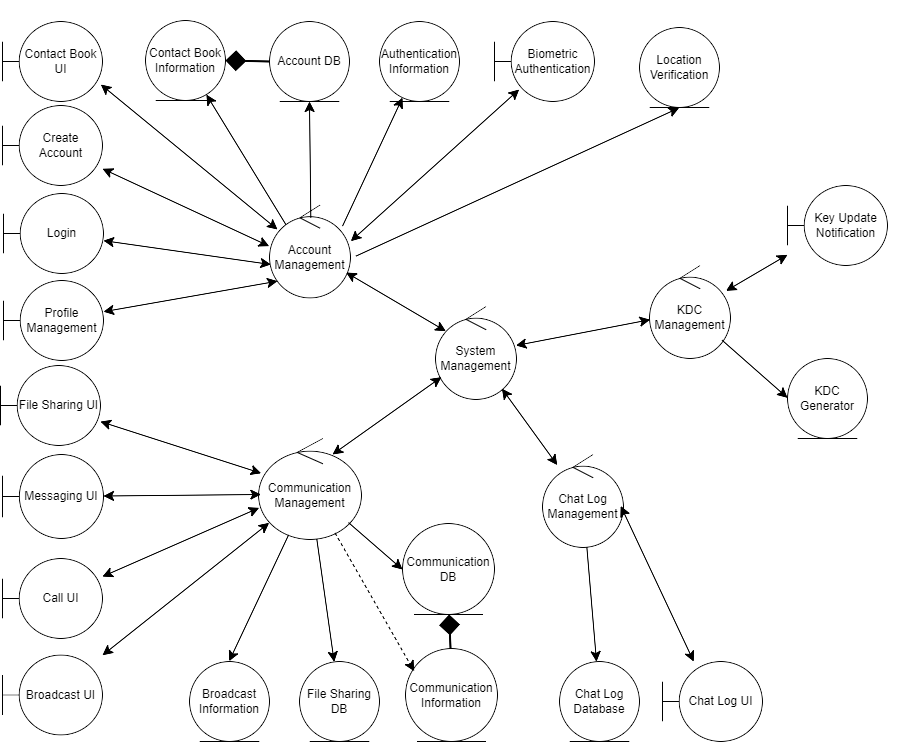
\includegraphics[width=\textwidth]{../images/ACD.png}

% End Section


\section{Architectural Design}
\label{sec:architectural_design}
% Begin Section
This section should provide an overview of the overall architectural design of your application. Your overall architecture should show the division of the system into subsystems with high cohesion and low coupling.

\subsection{System Architecture}
\label{sub:system_architecture}
% Begin SubSection
\begin{itemize}
	\item Identify and explain the overall architecture of your system
	\item Be sure to clearly state the name of the architecture you used (this is the name of the architectural pattern, not the name of your system)
	\item Provide the reasoning and justification of the choice of architecture
	\item Provide a structural architecture diagram showing the relationship among the subsystems (if appropriate)
	\item List any design alternatives you considered, but eliminated (and explain why you eliminated them)
\end{itemize}

There a 3 primary subsections within the system that utilize their own distinct architecture style but still exist within the overall larger architecture style:
\begin{center}
	\begin{tabular}{|p{2in} | p{2in}| p{2in}|}
		\hline
		Subsystem                & Purpose                                                                  & Architectural Style \\
		\hline
		Account Management       & Create, Login and Manage Account Information and Functions               & Repository          \\
		\hline
		Communication Management & Provides communication functionality between different agents and users. & Repository          \\
		\hline
		KDC Management           & Provides encryption and decryption functionalities                       & Pipe and Filter     \\
		\hline
	\end{tabular}
\end{center}

The subsystems employ the Repository and the Pipe and Filter architecture styles and the relationship and functionality are further defined in section 3.2.
\newline
\newline
We also include 4 databases on the model level, an account database, a contacts database, a KDC database and a Chat Log database.
\newline
\newline
-Talk about MVC Here
\newline
\newline
We chose the Repository Architecture Style for the Account Management and Communication Management subsystem since it supports easy scalability and utilizes a passive data store meaning the agents are active in controlling the data flow logic. This enables different agents to access different aspects of the system and different parts of data at the same time which will be beneficial for our system. Also having easy scalability through the introduction of new agents is crucial for our use case and easily implemented through this architecture style.
\newline
\newline
The Pipe and Filter Architecture Style was chosen for the KDC since it provides efficient processing of data with a high throughput and flexibility. Since we are expecting many messages at the same time throughput is a crucial factor to consider and the pipe and filter architecture allows for easy scaling of throughput through concurrency. It also provides simplicity by sectioning different parts of the KDC into filters for encryption and decryption. Finally it also allows for reusability and room to expand by simplify modifying or adding more pipes and filters.
\begin{center}
	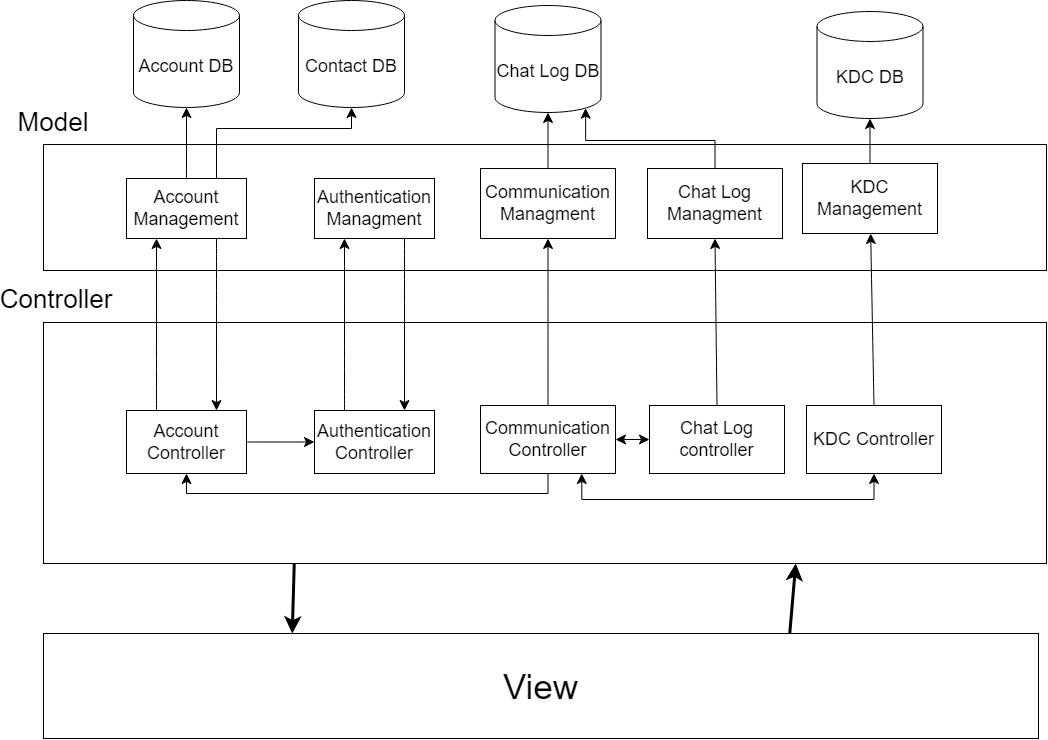
\includegraphics[width=0.7\paperwidth]{Systemarch.png}

\end{center}
% End SubSection

\subsection{Subsystems}
\label{sub:subsystems}
% Begin SubSection
Provide a list of your subsystems, with a brief description of each. Be sure to document its purpose and relationship to other subsystems.
\newline
\newline
We have 3 primary subsystems that are contained within the overall system which provide distinct functionalities and which also have their own distinct architectural styles for implementation. Our Three distinct subsytems include: Account Management, Communication Management Service, and KDC Managment.
\newline
\newline
The Account Management subsystem provides users with ability to create and login to their account and is responsible for ensuring that only authorized users account access the system by interfacing with the external apis. It also manages users contacts and interfaces with the communication management service to allow for communication and the authentication management for authentication management. It utilizes the repository architecture style.
\newline
\newline
The Communication Management Service provides users with the ability to contact other authorized user by sending and recieving messages. It also allows for the sending and recieving of files through file transfer, the reporting of messages and recieving of announcement board posts. It interacts with the authentication managment to ensure the authentication of users, the KDC Management for encryption and decryption of messages and the chat log managment and adheres to the Repository architecture style.
\newline
\newline
The KDC Management provides the encryption and decryption functions for the system. It interacts with the communication module and utilizes a pipe and filter architecture style.
% End SubSection

% End Section

\section{Class Responsibility Collaboration (CRC) Cards}
\label{sec:class_responsibility_collaboration_crc_cards}

\begin{table}[ht]
	\centering
	\begin{tabular}{|p{7cm}|p{7cm}|}
		\hline
		\multicolumn{2}{|l|}{\textbf{Class Name:} System Management (Controller)} \\
		\hline
		\textbf{Responsibility:}       & \textbf{Collaborators:}                  \\
		\hline
		Knows Account Management       & Account Management                       \\
		Knows Communication Management & Communication Management                 \\
		Knows Chat Log Management      & Chat Log Management                      \\
		Knows KDC Management           & KDC Management                           \\
		\hline
	\end{tabular}
\end{table}

\begin{table}[ht]
	\centering
	\begin{tabular}{|p{7cm}|p{7cm}|}
		\hline
		\multicolumn{2}{|l|}{\textbf{Class Name:} Communication Management (Controller)} \\
		\hline
		\textbf{Responsibility:}        & \textbf{Collaborators:}                        \\
		\hline
		Knows System Management         & System Management                              \\
		Knows File Sharing UI           & File Sharing UI                                \\
		Knows Call UI                   & Call UI                                        \\
		Knows Broadcast UI              & Broadcast UI                                   \\
		Knows Broadcast Information     & Broadcast Information                          \\
		Knows File Sharing DB           & File Sharing DB                                \\
		Knows Communication Information & Communication Information                      \\
		Knows Communication DB          & Communication DB                               \\
		\hline
	\end{tabular}
\end{table}

\begin{table}[ht]
	\centering
	\begin{tabular}{|p{7cm}|p{7cm}|}
		\hline
		\multicolumn{2}{|l|}{\textbf{Class Name:} File Sharing UI (Boundary)}     \\
		\hline
		\textbf{Responsibility:}                       & \textbf{Collaborators:}  \\
		\hline
		Knows Communication Management                 & Communication Management \\
		Handles the User Interface for file sharing    &                          \\
		Handles the encryption and decryption of files &                          \\
		\hline
	\end{tabular}
\end{table}

\begin{table}[ht]
	\centering
	\begin{tabular}{|p{7cm}|p{7cm}|}
		\hline
		\multicolumn{2}{|l|}{\textbf{Class Name:} Messaging UI (Boundary)}           \\
		\hline
		\textbf{Responsibility:}                          & \textbf{Collaborators:}  \\
		\hline
		Knows Communication Management                    & Communication Management \\
		Handles the User Interface for messaging          &                          \\
		Handles the encryption and decryption of messages &                          \\
		\hline
	\end{tabular}
\end{table}

\begin{table}[ht]
	\centering
	\begin{tabular}{|p{7cm}|p{7cm}|}
		\hline
		\multicolumn{2}{|l|}{\textbf{Class Name:} Call UI (Boundary)}             \\
		\hline
		\textbf{Responsibility:}                       & \textbf{Collaborators:}  \\
		\hline
		Knows Communication Management                 & Communication Management \\
		Handles the User Interface for calls           &                          \\
		Handles the encryption and decryption of calls &                          \\
		\hline
	\end{tabular}
\end{table}

\begin{table}[ht]
	\centering
	\begin{tabular}{|p{7cm}|p{7cm}|}
		\hline
		\multicolumn{2}{|l|}{\textbf{Class Name:} Broadcast UI (Boundary)}             \\
		\hline
		\textbf{Responsibility:}                            & \textbf{Collaborators:}  \\
		\hline
		Knows Communication Management                      & Communication Management \\
		Handles the User Interface for broadcasts           &                          \\
		Handles the encryption and decryption of broadcasts &                          \\
		\hline
	\end{tabular}
\end{table}

\begin{table}[ht]
	\centering
	\begin{tabular}{|p{7cm}|p{7cm}|}
		\hline
		\multicolumn{2}{|l|}{\textbf{Class Name:} Broadcast Information (Entity)} \\
		\hline
		\textbf{Responsibility:}                    & \textbf{Collaborators:}     \\
		\hline
		Knows Communication Management              & Communication Management    \\
		Knows what users belong to broadcasts       &                             \\
		Knows which users can message in broadcasts &                             \\
		\hline
	\end{tabular}
\end{table}

\begin{table}[ht]
	\centering
	\begin{tabular}{|p{7cm}|p{7cm}|}
		\hline
		\multicolumn{2}{|l|}{\textbf{Class Name:} File Sharing DB (Entity)}             \\
		\hline
		\textbf{Responsibility:}                             & \textbf{Collaborators:}  \\
		\hline
		Knows Communication Management                       & Communication Management \\
		Knows what users sent which files                    &                          \\
		Knows which users can view individual files          &                          \\
		Knows where all files that have been sent are stored &                          \\
		\hline
	\end{tabular}
\end{table}

\begin{table}[ht]
	\centering
	\begin{tabular}{|p{7cm}|p{7cm}|}
		\hline
		\multicolumn{2}{|l|}{\textbf{Class Name:} Communication Information (Entity)} \\
		\hline
		\textbf{Responsibility:}                    & \textbf{Collaborators:}         \\
		\hline
		Knows Communication Management              & Communication Management        \\
		Knows what users belong to which chat       &                                 \\
		Knows which users can message in which chat &                                 \\
		\hline
	\end{tabular}
\end{table}

\begin{table}[ht]
	\centering
	\begin{tabular}{|p{7cm}|p{7cm}|}
		\hline
		\multicolumn{2}{|l|}{\textbf{Class Name:} Chat Log Management (Controller)} \\
		\hline
		\textbf{Responsibility:} & \textbf{Collaborators:}                          \\
		\hline
		Knows System Management  & System Management                                \\
		Knows Chat Log Database  & Chat Log Management                              \\
		Knows Chat Log UI        & Chat Log UI                                      \\
		\hline
	\end{tabular}
\end{table}

\begin{table}[ht]
	\centering
	\begin{tabular}{|p{7cm}|p{7cm}|}
		\hline
		\multicolumn{2}{|l|}{\textbf{Class Name:} Chat Log Database (Entity)}                               \\
		\hline
		\textbf{Responsibility:}                                                  & \textbf{Collaborators:} \\
		\hline
		Knows Chat Log Management                                                 & Chat Log Management     \\
		Knows what user sent each message                                         &                         \\
		Knows the identifiers of users and the date, time, and content of message &                         \\
		\hline
	\end{tabular}
\end{table}

\begin{table}[ht]
	\centering
	\begin{tabular}{|p{7cm}|p{7cm}|}
		\hline
		\multicolumn{2}{|l|}{\textbf{Class Name:} Chat Log UI (Boundary)} \\
		\hline
		\textbf{Responsibility:}          & \textbf{Collaborators:}       \\
		\hline
		Knows Chat Log Management         & Chat Log Management           \\
		Handles presentation of Chat Logs &                               \\
		\hline
	\end{tabular}
\end{table}

% End Section


\appendix
\section{Division of Labour}
\label{sec:division_of_labour}
% Begin Section
Include a Division of Labour sheet which indicates the contributions of each team member. This sheet must be signed by all team members.
% End Section


\end{document}
%------------------------------------------------------------------------------